\section{Текст программы}

\lstinputlisting[language=Matlab]{../../src/lab01.m}


\section{Результат работы программы}
\begin{align*}
	M_{\max}          &= -2.45; \\
	M_{\min}          &= -7.26; \\
	R                 &= 4.81;  \\
	\hat\mu(\vec x_n) &= -4.76; \\
	S^2(\vec x_n)     &= 0.81;  \\
	m                 &= 8;		\\
	[ -7.26 ; -6.66 ) &- 3\:elements	\\
	[ -6.66 ; -6.06 ) &- 4\:elements	\\
	[ -6.06 ; -5.46 ) &- 20\:elements	\\
	[ -5.46 ; -4.86 ) &- 29\:elements	\\
	[ -4.86 ; -4.25 ) &- 30\:elements	\\
	[ -4.25 ; -3.65 ) &- 21\:elements	\\
	[ -3.65 ; -3.05 ) &- 10\:elements	\\
	[ -3.05 ; -2.45 ] &- 3\:elements	\\
\end{align*}


\section{Графики}
\begin{figure}[pt!]
	\centering
	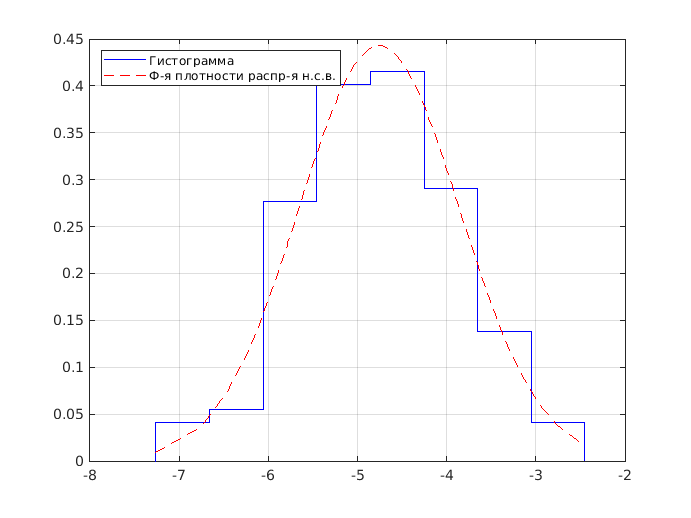
\includegraphics{../img/figure1}
	\caption{Гистограмма и график функции плотности распределения вероятностей нормальной случайной величины}
\end{figure}

\begin{figure}[pt!]
	\centering
	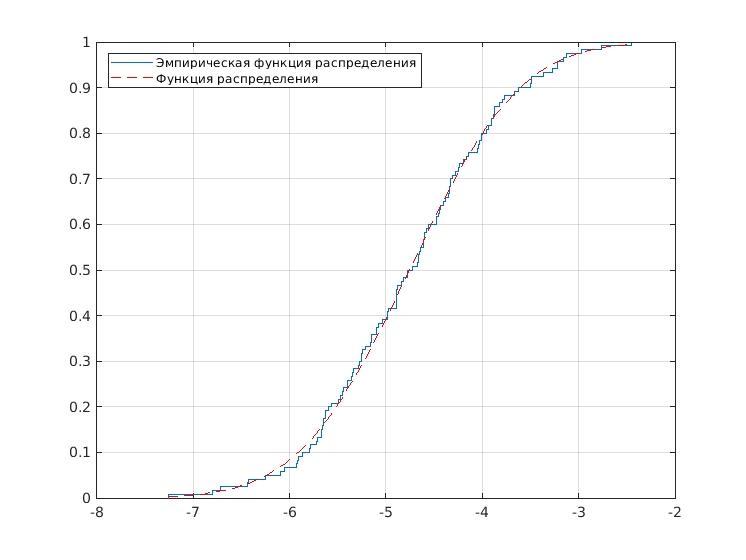
\includegraphics{../img/figure2}
	\caption{Эмпирическая функция распределения и функция распределения нормальной случайной величины}
\end{figure}